\section{TCP}

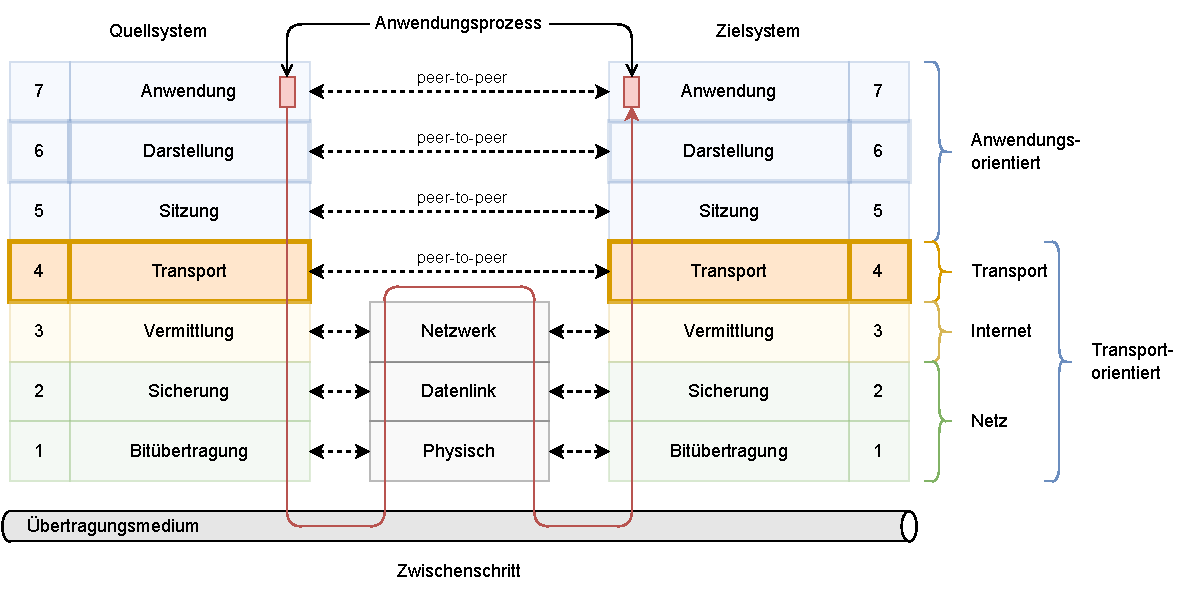
\includegraphics[width=\textwidth]{includes/figures/defi_iso_osi_transport.pdf}

\begin{defi}{TCP}
    Das \emph{Transmission Control Protocol (TCP)}  ist ein Netzwerkprotokoll, das definiert, auf welche Art und Weise Daten zwischen Netzwerkkomponenten ausgetauscht werden sollen.

    Das Protokoll ist ein \emph{zuverlässiges, verbindungsorientiertes, paketvermitteltes} Transportprotokoll in Computernetzwerken.

    Im Unterschied zum verbindungslosen UDP stellt TCP eine Verbindung zwischen zwei Endpunkten einer Netzverbindung (Sockets) her.
    Auf dieser Verbindung können in beide Richtungen Daten übertragen werden.

    TCP setzt in den meisten Fällen auf das IP (Internet-Protokoll) auf, weshalb häufig (und oft nicht ganz korrekt) auch vom TCP/IP-Protokoll die Rede ist.
    In Protokollstapeln wie dem OSI-Modell sind TCP und IP nicht auf derselben Schicht angesiedelt.

    TCP ist eine Implementierung der Transportschicht.

    Aufgrund seiner vielen positiven Eigenschaften (Datenverluste werden erkannt und automatisch behoben, Datenübertragung ist in beiden Richtungen möglich, Netzüberlastung wird verhindert usw.) ist TCP ein sehr weit verbreitetes Protokoll zur Datenübertragung.
    Beispielsweise wird TCP als fast ausschließliches Transportmedium für das WWW, E-Mail und viele andere populäre Netzdienste verwendet.
\end{defi}

\begin{defi}{TCP-Header}
    \begin{center}
        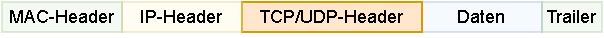
\includegraphics[width=0.75\textwidth]{includes/figures/defi_tcp_header_kapselung.pdf}

        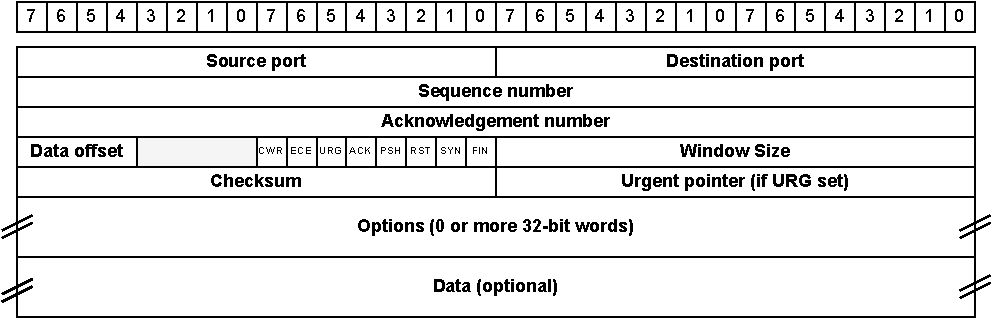
\includegraphics[width=0.75\textwidth]{includes/figures/defi_tcp_header.pdf}
    \end{center}
\end{defi}


\begin{defi}{Bestätigungen in TCP}
    Um empfangene Pakete zu bestätigen, wird eine \emph{Huckepack-Technik} verwendet; das bedeutet, dass Bestätigungen im Datenpaket der Rückrichtung erfolgen.

    Dabei kann eine Bestätigungsnachricht mehrere erhaltene Segmente bestätigen.

    Auch ohne Datenfluss in die Rückrichtung werden Bestätigungen verschickt, wenn auch oft verzögert.\footnote{Nach 500ms muss eine Bestätigung verschickt werden. Nach zwei vollständigen Segmenten sollte ebenfalls eine Bestätigung verschickt werden.}
    Diese verzögerten Bestätigungen heißen \emph{Delayed Acknowledgments}.

    Es gilt:

    \begin{tabularx}{\textwidth}{|X|X|}
        \hline
        Ereignis beim Empfänger                                                                                                             & Aktion beim Empfänger                                                                                                  \\
        \hline
        \hline
        Ankunft eines Segments mit der erwarteten Sequenznummer. Alle Daten bis dahin sind schon bestätigt worden.                          & Delayed ACK. Warte bis zu 500ms auf das nächste Segment. Wenn dieses nicht empfangen wird, verschicke die Bestätigung. \\
        \hline
        Ankunft eines Segments mit der erwarteten Sequenznummer. Allerdings wurde noch keine Bestätigung des voherigen Segments verschickt. & Sofortiges Verschicken einer kumulativen Bestätigung, die beide Segmente bestätigt.                                    \\
        \hline
        Ankunft eines Segments hinter der erwarteten Sequenznummer. Es wird eine Lücke entdeckt.                                            & Sofortiges Verschicken eines Duplicate ACK (\texttt{Dup ACK}). Diese enthält erneut die erwartete Segmentnummer.       \\
        \hline
        Ankunft eines Segments, das eine Lücke teilweise oder vollständig füllt.                                                            & Sofortiges Verschicken einer Bestätigung.                                                                              \\
        \hline
    \end{tabularx}
\end{defi}

\begin{example}{Bestätigungen in TCP}
    \begin{center}
        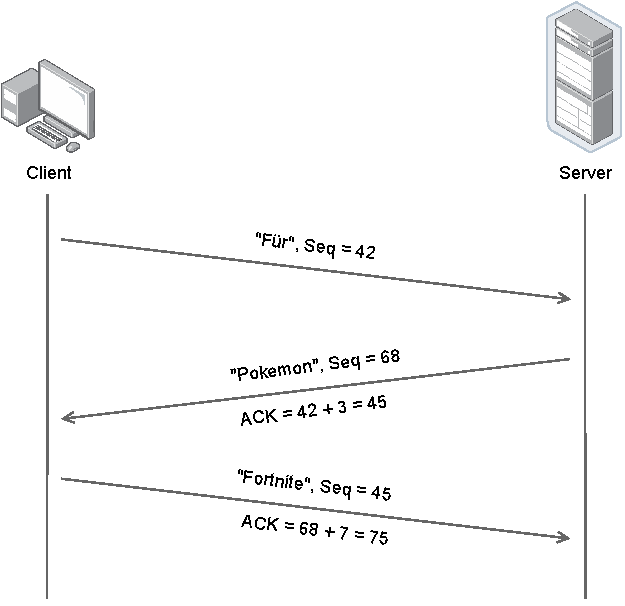
\includegraphics[width=0.5\textwidth]{includes/figures/example_ack.pdf}
    \end{center}
\end{example}

\begin{example}{Delayed Acknowledgments}
    \begin{center}
        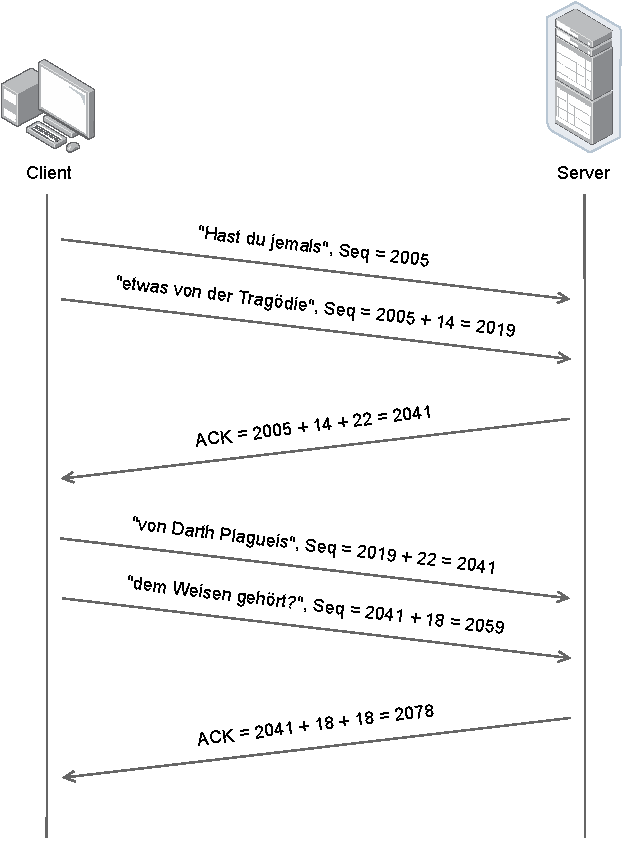
\includegraphics[width=0.5\textwidth]{includes/figures/example_delayed_ack.pdf}
    \end{center}
\end{example}

\begin{bonus}{Go-Back-N}
    \emph{Go-Back-N} stellt ein Verfahren dar, das im Gegensatz zu Stop-and-Wait einen deutlich größeren Durchsatz ermöglicht.

    Der Sender kann dabei mehrere Dateneinheiten senden, ohne auf eine Quittung warten zu müssen.
    Wie viele das sind, hängt von der sogenannten \emph{Fenstergröße} ab.

    Beträgt diese $n$, kann der Sender noch $n-1$ weitere Dateneinheiten absenden, bevor die Bestätigung für die erste Einheit durch den Empfänger erfolgt sein muss.

    Es können vom Empfänger auch mehrere Dateneinheiten auf einmal (kumulativ) bestätigt werden, so zeigt eine Quittung für $n+i$ an, dass alle Einheiten von $n$ bis $n+i$ korrekt empfangen wurden.

    Kommt es beim Warten auf die Bestätigungen zu einem Timeout, so übermittelt der Sender alle Dateneinheiten in dem Fenster neu.
    Er geht also zurück zur letzten unbestätigten Sequenznummer $N$.

    Da es der Fall sein kann, dass lediglich eine Dateneinheit nicht ordnungsgemäß übertragen wurde und dennoch auch alle danach gesendeten erneut übertragen werden, wird an dieser Stelle Übertragungskapazität verschwendet.
\end{bonus}

\begin{bonus}{Selecive-Repeat}
    Bei \emph{Selective Repeat}  wird ein fehlerhafter Rahmen verworfen, aber die danach erhaltenen Rahmen werden im Empfänger in einem Puffer abgelegt und bestätigt.

    Wenn beim Sender die Zeit abgelaufen ist, wird nur der älteste nicht bestätigte Rahmen erneut übertragen.
    Wenn dieser Rahmen korrekt ankommt, kann der Empfänger in der Folge alle im Puffer gespeicherten Rahmen an die Vermittlungsschicht übergeben.

    Die selektive Wiederholung wird oft mit dem Senden einer negativen Bestätigung (\texttt{NAK}, \emph{Negative Acknowledgement}) durch den Empfänger kombiniert, wenn dieser einen Fehler wie einen Prüfsummenfehler oder einen Rahmen außerhalb der Reihenfolge entdeckt.

    \texttt{NAKs} stoßen die erneute Übertragung an, bevor der entsprechende Timer abläuft und verbessern daher die Leistung.
\end{bonus}

\begin{defi}{Round Trip Time}
    Die \emph{Round Trip Time (RTT)} gibt die Zeit an, die ein Datenpaket (Datagramm) in einem Rechnernetz benötigt, um von der Quelle zum Ziel und zurück zu reisen.

    Es handelt sich also um die Summe aus Laufzeit von Punkt A nach Punkt B und der Laufzeit von Punkt B nach Punkt A.

    Die RTT wird zum Beispiel vom Transmission Control Protocol (TCP) laufend gemessen, um zu bestimmen, wann Pakete nach Ausbleiben einer Bestätigung erneut gesendet werden sollten.
\end{defi}

\begin{bonus}{Slow-Start}
    Zu Beginn einer Datenübertragung dient der \emph{Slow-Start-Algorithmus} zur Bestimmung des Überlastfenster (\emph{congestion window}), um einer möglichen Überlastsituation vorzubeugen.

    Der Algorithmus startet mit einem kleinen Fenster von einer MSS (Maximum Segment Size), in dem Datenpakete vom Sender zum Empfänger übertragen werden.

    Der Empfänger sendet nun eine Bestätigung (\texttt{ACK}) an den Sender zurück.
    Für jedes empfangene \texttt{ACK} wird die Größe des congestion window um eine MSS erhöht.
    Da für jedes versandte Paket bei erfolgreicher Übertragung ein \texttt{ACK} geschickt wird, führt dies innerhalb einer Roundtrip-Zeit zu einer Verdopplung des Congestion Windows.
    In dieser Phase gibt es also ein exponentielles Wachstum.

    Dieses exponentielle Wachstum wird so lange fortgesetzt, bis der sogenannte \emph{Slow-Start Threshold} erreicht wird.\footnote{Die Phase des exponentiellen Wachstums wird auch Slow Start Phase genannt.}

    Danach wird das Congestion Window nur noch um eine MSS erhöht, wenn alle Pakete aus dem Fenster erfolgreich übertragen wurden.\footnote{Es wächst also pro Roundtrip-Zeit nur noch um eine MSS, also nur noch linear. }
    Diese Phase wird als Congestion Avoidance Phase bezeichnet.

    Das Wachstum wird beendet, wenn das vom Empfänger festgelegte Empfangsfenster erreicht worden ist.

    Kommt es zu einem Timeout, wird das congestion window wieder auf 1 zurückgesetzt, und der slow-start threshold wird auf die Hälfte der \emph{Flight Size}\footnote{Flight Size ist die Anzahl an Paketen, die verschickt, aber noch nicht quittiert wurden.} herabgesetzt.
    Die Phase des exponentiellen Wachstums wird also verkürzt, so dass das Fenster bei häufigen Paketverlusten nur langsam wächst.
\end{bonus}

\begin{defi}{TCP-Verbindungsmanagement (Verbindungsaufbau)}
    Der Client, der eine Verbindung aufbauen will, sendet dem Server ein \texttt{SYN}-Paket mit einer Sequenznummer $x$.
    Die Sequenznummern sind dabei für die Sicherstellung einer vollständigen Übertragung in der richtigen Reihenfolge und ohne Duplikate wichtig.

    Die Start-Sequenznummer ist eine beliebige Zahl, deren Generierung von der jeweiligen TCP-Implementierung abhängig ist.
    Sie sollte jedoch möglichst zufällig sein, um Sicherheitsrisiken zu vermeiden.

    Der Server empfängt das Paket. Ist der Port geschlossen, antwortet er mit einem \texttt{TCP-RST}, um zu signalisieren, dass keine Verbindung aufgebaut werden kann.

    Ist der Port geöffnet, bestätigt er den Erhalt des ersten \texttt{SYN}-Pakets und stimmt dem Verbindungsaufbau zu, indem er ein \texttt{SYN/ACK}-Paket zurückschickt.
    Zusätzlich sendet er im Gegenzug seine Start-Sequenznummer y, die ebenfalls beliebig und unabhängig von der Start-Sequenznummer des Clients ist.

    Der Client bestätigt zuletzt den Erhalt des \texttt{SYN/ACK}-Pakets durch das Senden eines eigenen \texttt{ACK}-Pakets mit der Sequenznummer x+1. Dieser Vorgang wird auch als \emph{Forward Acknowledgement} bezeichnet.
    Aus Sicherheitsgründen sendet der Client den Wert $y+1$ im \texttt{ACK}-Segment zurück.

    \centering
    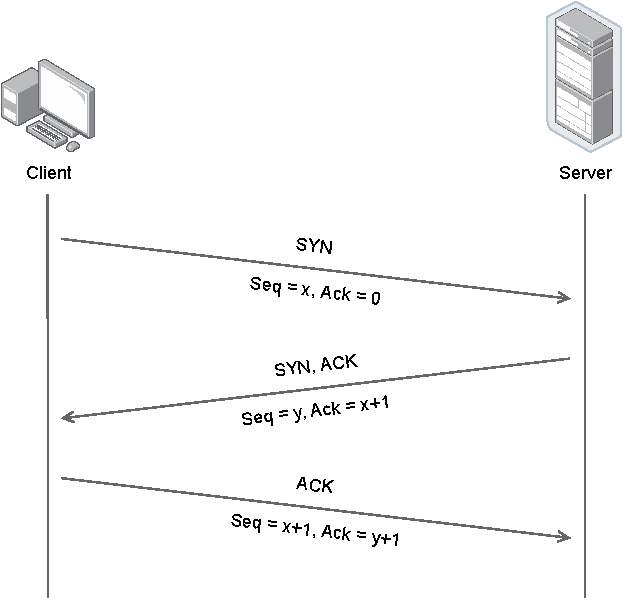
\includegraphics[width=0.5\textwidth]{includes/figures/defi_tcp_verbindungsaufbau.pdf}
\end{defi}

\begin{defi}{TCP-Verbindungsmanagement (Verbindungsende)}
    Statt des \texttt{SYN}-Bits kommt das \texttt{FIN}-Bit  zum Einsatz, welches anzeigt, dass keine Daten mehr vom Sender kommen werden.
    Der Erhalt des Pakets wird wiederum mittels \texttt{ACK} bestätigt.

    Der Empfänger des \texttt{FIN}-Pakets sendet zuletzt seinerseits ein \texttt{FIN}-Paket, das ihm ebenfalls bestätigt wird.

    \centering
    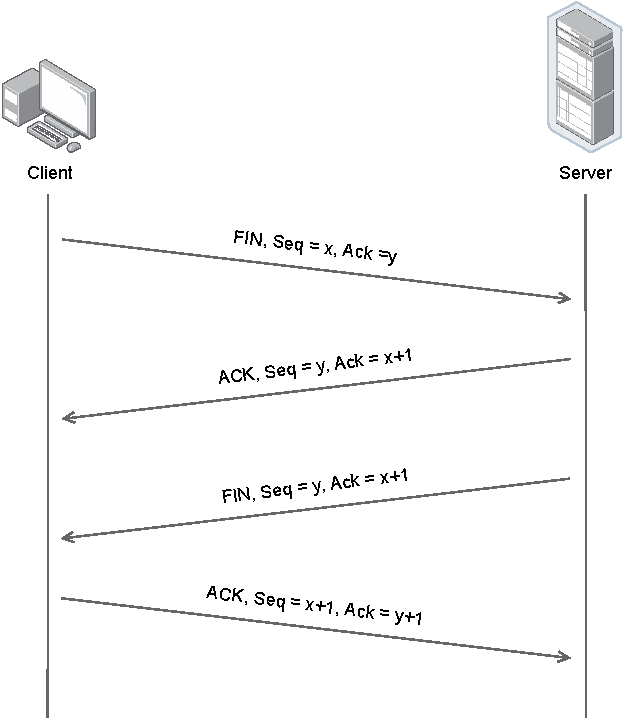
\includegraphics[width=0.5\textwidth]{includes/figures/defi_tcp_verbindungsabbau.pdf}
\end{defi}

\begin{defi}{Flusskontrolle}
    Die \emph{Flusskontrolle (Flow Control)}, ist eine Funktion von Kommunikationsprotokollen zur Anpassung der Übertragungsgeschwindigkeit asynchron arbeitender Endgeräte an die Aufnahmefähigkeit der empfangenden Station.

    Die Flusskontrolle regelt die Datenrate zwischen der sendenden und empfangenden Station und sorgt für eine Geschwindigkeitsadaption und dafür, dass die Datenübertragung verlustfrei erfolgt.

    Bei Überlast der Übertragungsstrecke oder bei Datenstau veranlasst das empfangende Endgerät das sendende dazu die Datenrate soweit zu reduzieren oder zeitweise auszusetzen, damit die empfangende Station alle Daten der sendenden Station aufnehmen kann.

    Eine Überlast tritt dann auf, wenn die Anzahl der Datenpakete, die eine sendende Station dem Netz übergibt, die Aufnahmekapazität der empfangendes Endgerätes überschreitet.
\end{defi}

\begin{defi}{Flusskontrolle in TCP}
    TCP implementiert das \emph{Sliding-Window-Protokoll}:
    \begin{itemize}
        \item Bei einer Fenstergröße von $n$ können $n$ Bytes verschickt werden, ohne dass ein \texttt{ACK} empfangen werden muss.
        \item Wenn der Empfang der Daten vom Empfänger bestätigt wurde, so verschiebt sich das Fenster.
    \end{itemize}

    Segmente werden durch ihren Byte-Offset im Stream identifiziert (\emph{Sequence Number}), wobei die Startposition beim Verbindungsaufbau zufällig festgelegt wird.

    TCP verwendet kumulative \texttt{ACKs}. $\texttt{ACK n+1}$ sagt aus, dass alle Daten von der vorherigen logischen Position bis zur Position $n$ korrekt empfangen wurden und nun das Segment $n+1$ erwartet wird.
\end{defi}

\begin{defi}{Sliding Window in TCP}
    Da die Anwendung Daten aus dem Puffer liest, ändert sich der Füllstand des Puffers ständig.
    Deshalb ist es notwendig, den Datenfluss dem Füllstand entsprechend zu steuern.
    Dies geschieht mit dem \emph{Sliding Window} und dessen Größe.

    Mit dem Window-Feld kann er dem Sender mitteilen, dass er keine Daten mehr verschicken soll.
    Dies geschieht, indem er im Window-Feld den Wert Null einträgt (Zero Window).
    Der Wert Null entspricht dem freien Speicherplatz im Puffer.
\end{defi}

\begin{example}{Sliding Window in TCP}
    \begin{center}
        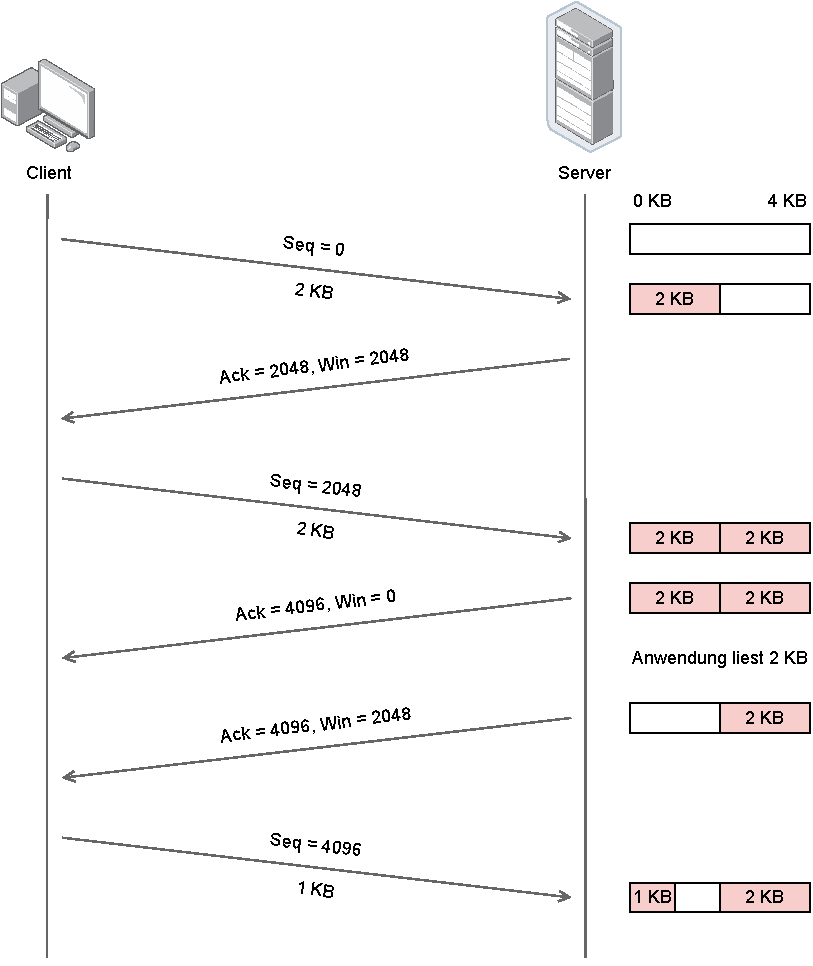
\includegraphics[width=0.75\textwidth]{includes/figures/example_tcp_window_management.pdf}
    \end{center}
\end{example}

\begin{bonus}{Silly Window Syndrome}
    Zuerst sendet der Empfänger ein Zero Window, weil sein Empfangspuffer voll ist.
    Nachdem die Anwendung einige Bytes (z.B. 4) aus dem Empfangspuffer gelesen hat, sendet der Empfänger ein Window Update mit \texttt{Window = 4} an den Sender.
    Der Sender sendet dadurch ein TCP-Segment mit lediglich vier Bytes Nutzlast.

    Dieses Verhalten setzt sich weiter so fort. Dadurch entsteht ein großer Protokoll-Overhead.

    Eine Lösung ist, dass der Empfänger ein Zero Window sendet und so lange mit dem Window Update warten soll, bis die Anwendung mindestens die maximale Segmentgröße (\emph{maximum segment size}) aus dem Puffer gelesen hat oder der Puffer halbleer ist – je nachdem, was zuerst eintritt.
\end{bonus}

\begin{defi}{TCP Receive Window}
    Die \emph{TCP Receive Window (Size)} ist neben der Maximum Segment Size (MSS) ein Parameter, der die Funktion des Netzwerkprotokolls TCP steuert.
    Sie beschreibt die maximale Datenmenge, die ein Computer empfangen kann, ohne Daten bestätigen zu müssen.

    Im Umkehrschluss ist es also die maximale Datenmenge, die ein Computer senden kann, ohne auf eine Empfangsbestätigung des Empfängers warten zu müssen.

    Damit ist sichergestellt, dass der Empfangsspeicher (Puffer) des Empfängers nicht überläuft, da dieser nie mehr Daten am Stück empfängt, als er dem Sender durch Übermittlung seiner aktuellen Empfangsfenstergröße erlaubt hat.
    Erst wenn der Empfänger Daten bestätigt (und damit aus dem Puffer entfernt) hat, sendet der Sender die nächsten Daten.
\end{defi}

\begin{bonus}{Retransmission Timer}
    Zur Feststellung, wann ein Paket im Netzwerk verloren gegangen ist, wird vom Sender ein Timeout verwendet, bis zu dem das \texttt{ACK} der Gegenseite eingetroffen sein muss.

    Ein zu niedriger Timeout bewirkt, dass Pakete, die eigentlich korrekt angekommen sind, wiederholt werden; ein zu hoher Timeout bewirkt, dass bei tatsächlichen Verlusten das zu wiederholende Paket unnötig spät gesendet wird.

    Aufgrund unterschiedlicher Laufzeiten der zugrundeliegenden IP-Pakete ist nur ein dynamisch an die Verbindung angepasster Timer sinnvoll.
\end{bonus}